\chapter{Introduction} \label{ch:introduction}
This thesis begins with notation that is used throughout this document.
\section{Notation}
Mathematical notations, some standard as well as some non-standard, are introduced here.

A tuple, which is dennoted by angle brackets $\langle \cdots \rangle$, is to be regarded as a column
vector. $\bm{1}$ denotes the column vector of all 1s. Superscript $T$ indicates transpose. 
The standard vector norm is $\|x\| \;=\; \sqrt{x^T x}$. Modulus (or absolute value) is denoted by $|\; \cdot \;|$. 
When $S$ is a set, $|S|$ denotes the cardinality of $S$.

The notation $O(f)$ denotes a function $g$ such that pointwise $g \;\leq \;c f$ for some constant $c$. 
The notation $\theta(f)$ is a function $g$ such that pointwise 
$c_0 f \;\leq\; g \;\leq\; c_1 f$ for some constants $c_0 \;,\; c_1$. 
Curly brackets $\{\cdots\}$ are used as grouping symbols and to specify both sets
and multisets. Square brackets $[ \cdots ]$ are used to specify 
a closed interval of real numbers as well as to denote {\em Iverson bracket}. 
{\em Iverson bracket} is an indicator function:
if $expr$ is an expression, then
$[\mbox{\em expr\/} ]$ denotes $1$ if {\em expr\/} is
true, and $0$ otherwise. 

{\em sup \/} indicates the supremum which is the least upper bound. {\em inf \/} indicates the infimum, 
that is, the greatest lower bound.

The set of length $\ell$ binary strings is denoted by $\mathcal{R}$. It is a
commutative ring under component-wise addition and
multiplication modulo $2$. If $x \in \mathcal{R}$, then it may 
be regarded as the vector $x = \langle x_0, x_1, \cdots, x_{\ell - 1} \rangle$. 
The additive identity of $\mathcal{R}$ is ${\bf 0}$ and the
multiplicative identity is ${\bf 1}$. Let $\overline{g}$
abbreviate ${\bf 1} + g$.  Except when explicitly indicated otherwise,
operations acting on elements of $\mathcal{R}$ are as defined in this
paragraph. In particular, $g \overline{g} = {\bf 0} = g+g$,
  $g^2 = g$, $g + \overline{g} = {\bf 1}$ for all $g \in
  \mathcal{R}$.


\section{Background}
\subsection{Genetic Algorithm}
The genetic algorithm (GA) is inspired by nature, and seeks to evolve useful constructs. It is typically population based, and 
proceeds over a number of generations to evolve solutions to problems not yielding to other known methods. 
Several people working in the 1950s and the 1960s -- like Box (1957), Friedman (1959),
Bledsoe (1961), Bremermann (1962), and Reed, Toombs and Baricelli (1967) -- developed evolution-inspired algorithms, 
but little attention or theoretical analysis was given to them (see \cite{Mitchell1999}). Genetic algorithms were popularized by Holland 
and his colleagues in the 1960s and the 1970s. Holland introduced a population-based algorithm with crossover and mutation, 
and promoted his schema theorem ( see \cite{Holland1975}). 
Basic elements of a simple style GA are: 
selection according to fitness, crossover, and random mutation (see \cite{Mitchell1999}). 
In the simplest case, population members are fixed-length binary strings.   
The fitness function assigns a value (fitness) to the elements (chromosomes) of 
the current population. 

\textit{Selection}: select population members in the current population for reproduction; 
those with higher fitness are more likely to be selected to reproduce.

\textit{Crossover}: with some probability (the crossover rate), choose a random point in two parents (population members selected for reproduction) 
and exchange subsequences after that point to create two offspring.

\textit{Mutation}: flip bits of an individual with some small probability, 
the mutation rate.

Figure \ref{FiniteGA} shows the procedural flow of a basic finite population genetic algorithm.
\begin{figure}[H]
\begin{center}
\resizebox*{8cm}{!}{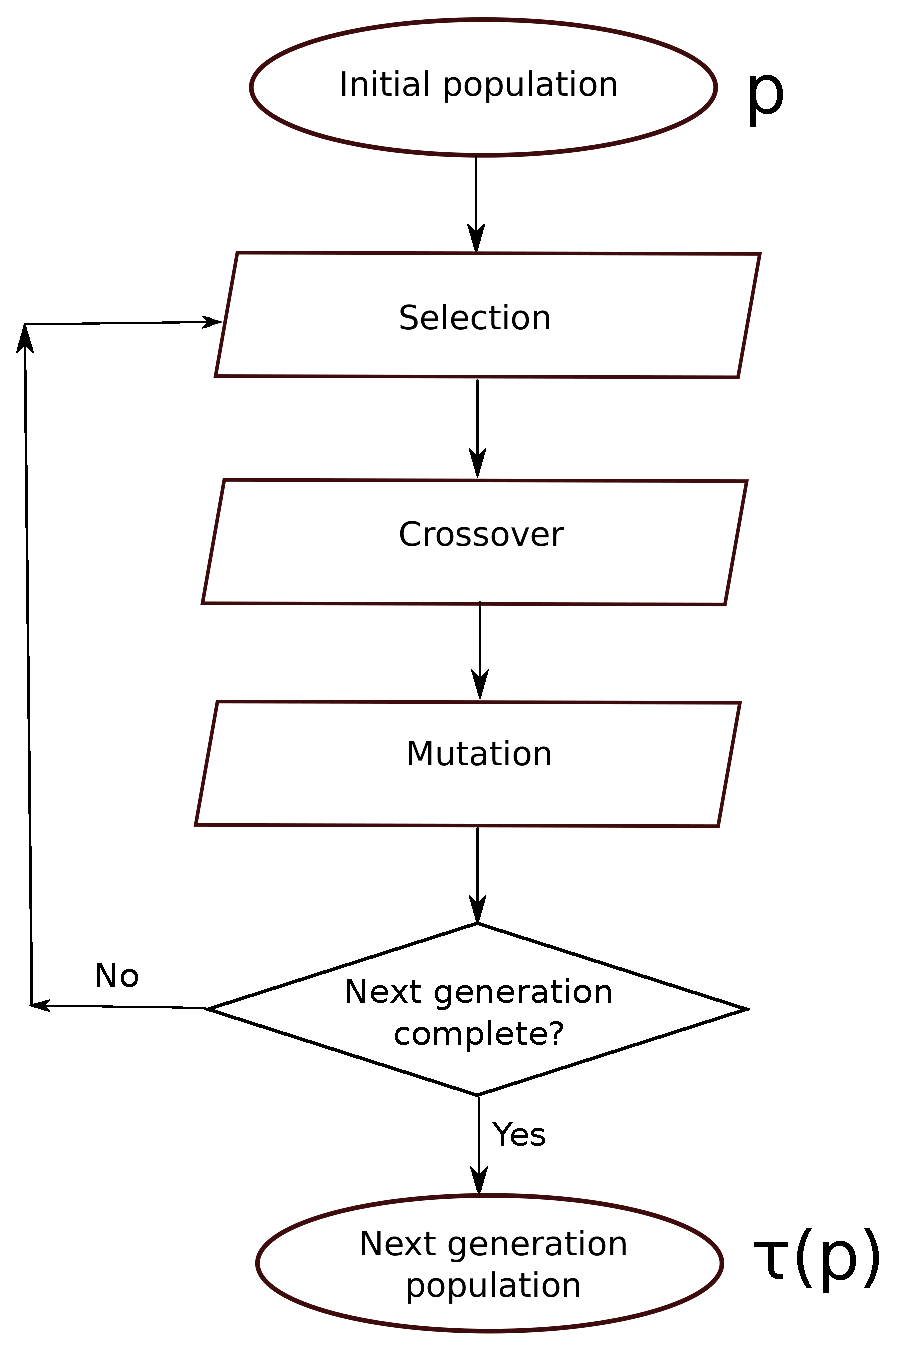
\includegraphics{figures/eps/GA.eps}}\hspace{4pt}
\caption{\textbf{Finite GA (Haploid)} }
\label{FiniteGA}
\end{center}
\end{figure}

A simple Holland style genetic algorithm:

\begin{algorithm}
\caption*{}
\begin{algorithmic}[1]
\Statex 1. Start with some population $P$ containing $r$ binary strings of length $\ell$
\Statex 2. Choose parents $u$ and $v$ from the current population $P$ (using any selection scheme with replacement)
  \Statex \hspace{\algorithmicindent} a. Crossover $u$ and $v$ to produce children $u^\prime$ and $v^\prime$
  \Statex \hspace{\algorithmicindent} b. Mutate $u^\prime$ and $v^\prime$ with some probability to produce $u^{\prime\prime}$ and $v^{\prime\prime}$
  \Statex \hspace{\algorithmicindent} c. Keep, with uniform probability, one of $u^{\prime\prime}$ and $v^{\prime\prime}$ for the next generation 
\Statex 3. Repeat step 2 until $r$ offspring are created
\Statex 4. Replace $P$ by the new generation formed and go to step 2
\end{algorithmic}
\label{RealGA}
\end{algorithm}

Each iteration of this process produces a generation. 
The process described above is repeated until the system stops to improve or some threshold is met. 

Figure \ref{FiniteGADip} illustrates 
algorithm for finite diploid population genetic algorithm. 
In case of diploid population GA each parent ($u$ or $v$) 
has two haploid components ($\langle u_0, u_1 \rangle$ or $\langle v_0, v_1 \rangle$). 
Instead of crossing over two parent diploids, 
haploids in each diploid $u_0$ and $u_1$, and $v_0$ and $v_1$ 
crossover and mutate to produce gametes $g_0$ and $g_1$ from  each diploid. 
And gametes $g_0$ and $g_1$ are fused to form offspring diploid $ \langle g_0, g_1 \rangle $.

\begin{figure}[H]
\begin{center}
\resizebox*{8cm}{!}{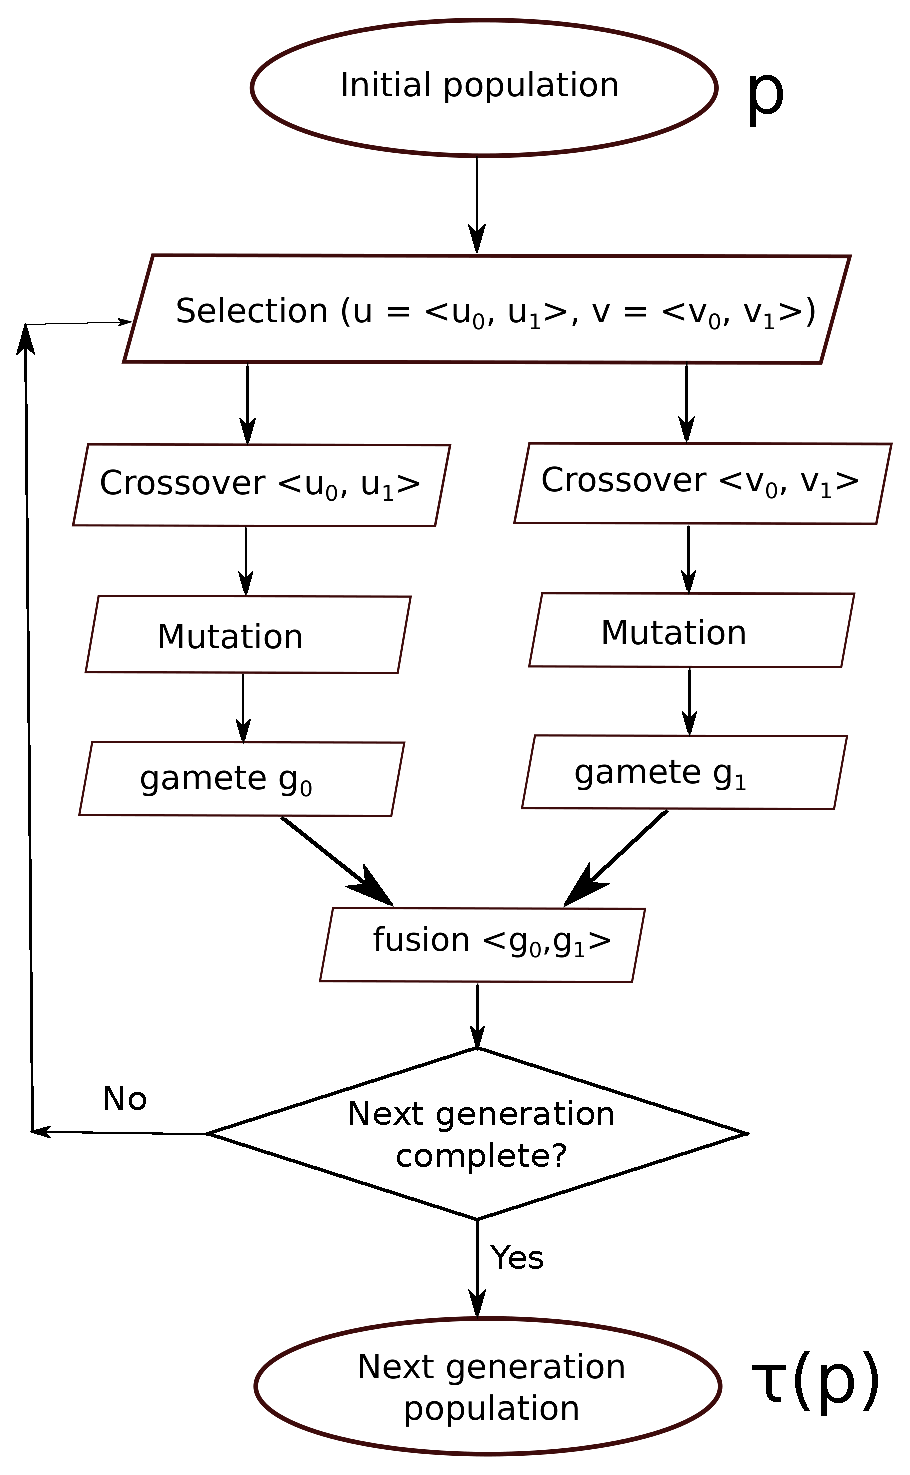
\includegraphics{figures/eps/GA_dip.eps}}\hspace{4pt}
\caption{\textbf{Finite GA (Diploid)} }
\label{FiniteGADip}
\end{center}
\end{figure}

\subsection{Infinite Population Model}
Haldane, in the classic book `The Causes Of Evolution', presents a summary of the basic models of population genetics 
by Wright, Fisher, and Haldane (see \cite{Haldane1932}). 
Holland introduced a population-based algorithm with crossover and mutation, 
and promoted his schema theorem as a theoretical means by which to analyze genetic algorithm dynamics ( see \cite{Holland1975}). 
Holland's Schema theorem provides a lower bound for schema survival in 
next generation.\footnote{A schema is a template that identifies a set of strings in the population with similarities 
at certain string positions; it is made up of $1$s, $0$s, and $\ast$s where 
$\ast$ is the 'don't care' symbol that matches either $0$ or $1$.} The schema theorem is an inequality however, 
and can not predict which strings are expected in the next generation. 
Bethke (see \cite{Bethke1981}) gave equations computing the expected number of any string in the next generation. 
Goldberg (see \cite{Goldberg1987}) used such equations 
to model the evolutionary trajectory of a two bit GA under crossover 
and proportional selection. Vose and Liepins (see \cite{VoseLiepins1991}) simplified and extended 
these equations by integrating mutation into the recombination of arbitrarily long binary strings. 
Although their model computes infinite population trajectories, given a {\em finite} population represented by vector $\bm{p}$  
(component $\bm{p}_i$ is the proportion of string $i$ in the {\em finite population}), the infinite population model 
computes the expected proportion $\mathcal{G}(\bm{p})_i$ of string $i$ in the next generation.  This is perhaps the most 
direct connection between the infinite population model and a finite population GA. In the model, $\mathcal{G}$ 
comprises of fitness matrix $F$ and recombination operator $\mathcal{M}$ that includes application of crossover and mutation.

The infinite population GA models a population as a vector $\bm{p}$ where component $\bm{p}_j$ 
can be interpreted as the proportion of string $j$ in the population. If $\mathcal{G}$ is the function mapping infinite population $\bm{p}$ to 
the next generation, $\mathcal{G}(\bm{p})$ is a vector such that 
\[
\mathcal{G}(\bm{p})_j \; = \; \text{proportion of $j$ in the next generation}.
\]
The evolution of infinite population $\bm{p}$ is the sequence
\[ \bm{p} \to \mathcal{G}(\bm{p}) \to  {\mathcal{G}}(\mathcal{G}(\bm{p})) \to \cdots \]
\setcounter{footnote}{2}

\subsection{Finite Population Model}
Infinite population model is assumption of perfection of genetic algorithm that simplifies analysis. However, finite population 
can behave very differently than predicted by infinite population model due to stochasticity involved and sampling errors. 
Nix and Vose (see \cite{Nix1992}) explored issues regarding the relationship between the finite population GA and the infinite population model. 
They showed, for a mutation rate $\mu$ between $0$ and $0.5$, a finite population GA will form an ergodic Markov chain, 
visiting every state infinitely often in the long run. Nix and Vose set up their Markov model with transition matrix $Q$ where 
$Q_{i,j}$ is probability that population $P_j$ will be produced from $P_i$. 
They showed that the short term trajectory followed by a finite population is related to 
the evolutionary path determined by the infinite population model, and  
for large populations, the short term trajectory follows closely and 
with large probability approaching 1, that path predicted by 
the infinite population model. 

Vose later extended both infinite population model and finite population model 
through general abstract search method Random Heuristic Search (RHS) (described more in section \ref{RHS}).
% So if we form a geometrical cylinder 
% around the path determined by the infinite population model, a finite population GA will stay inside the pipe in the short term, and 
% then escape it after some period of time. 

% Vose and Liepins apply Walsh transform to mixing to analyse and get results. 
% With Markov chain modeling of simple GA, Vose and Nix (see \cite{Nix1992}) investigated asymptotic behavior of steady 
% state distributions as population size increases and showed that if finite population is sufficiently large, 
% convergence behavior of a real GA can be predicted. As population size increases, the correspondence improves 
% between expected population predicted using infinite population model and the actual population observed in 
% finite population genetic algorithm. 

\subsection{Walsh Transform}
Vose compiled and extended previous work regarding the infinite population model in the book 
\textit{Simple Genetic Algorithm: Foundations and Theory} (see \cite{Vose1999}). 
In particular, he discussed how the Walsh transform can be applied to increase 
computational efficiency in calculations related to the infinite population model. 
There have been previous applications of the Walsh transform to GAs. Bethke first introduced the 
idea of using Walsh transforms to analyze GA fitness functions in terms of schemata (see \cite{Bethke1981}). 
The idea was further developed in papers by Goldberg (see \cite{Goldberg1989a}, \cite{Goldberg1989b}). 
However, such usage did not apply Walsh transforms  to crossover, to mutation, or to any of their 
associated mathematical objects. In contrast, Vose and Liepins applied the Walsh transform directly to mutation and recombination, and proved that the 
twist $M^\ast$ of the mixing matrix $M$ is triangularized by the Walsh transform, and 
related eigenvalues of $M^\ast$ to the stability of fixed points of $\mathcal{G}$ (see \cite{VoseLiepins1991}).\footnote{The mixing 
matrix $M$ has rows and columns indexed by chromosomes; entry $M_{i,j}$ is the probability 
that mixing parents $i$ and $j$ (mixing is the combined effect of crossover and mutation) will produce a 
child having all bits zero. The twist $(M^\ast)$ of the mixing matrix $M$ is defined by $(M^\ast)_{i,j} = M_{i+j, i}$.} 
In a related paper, Koehler (see \cite{Koehler1994}) gives a congruence 
transformation defined by a lower triangular matrix that diagonalizes the mixing matrix (for 1-point crossover and mutation 
given by a rate) and proved a conjecture of Vose and Liepins concerning eigenvalues of $M^\ast$. Koehler, Bhattacharyya 
and Vose (see \cite{KoehlerBhatta1997}) applied the Fourier transform in generalizing results established 
for binary GAs to 
strings over an alphabet of cardinality $c$ (in the binary case, the Fourier transform is the Walsh transform). 
From a computational perspective, a major contribution of Vose and Wright (see \cite{VoseWright1998}) was demonstrating that 
the mixing matrix is sparse in the Walsh basis, and the computational efficiency of 
computing $\mathcal{G}(\bm{p})$ can thereby be improved from 
$O(8^\ell)$ to $O(3^\ell)$ where $\ell$ is the chromosome length. The cost of moving from standard coordinates to the Walsh basis need not be a bottleneck; 
the fast Walsh transform (see \cite{Shanks1969}) does that in $O(\ell \, 2^\ell)$ time.

\section{Random Heuristic Search}
\label{RHS}
The work presented in this thesis is based on {\em Random Heuristic Search (RHS)}, 
a general search method, defined upon the central concept of state and transition 
between states (see \cite{Vose1999}). The simple genetic algorithm is a particular type of RHS. 
An instance of {\em RHS} is an initial collection of elements $P$ (referred to as the initial population) chosen 
from some search space $\Omega$, together with a stochastic transition rule $\tau$, which from $P$ will 
produce another collection $P^\prime$; iterating $\tau$ produces a sequence of generations.

Let $n$ be the cardinality 
of $\Omega$, let ${\bf1}$ denote the column vector of all 1s. 
The set of population descriptors is termed as  {\em simplex}:
\[
\Lambda = \{x = \langle x_0,...,x_{n-1} \rangle: {\bf1}^T x=1, x_j \geq 0 \} %\text{\footnotemark\label{fnm:1}}
\]
%\footnotetext{$\langle .. \rangle$ represents a column vector; ${\bf1}$ is $\langle 1,..,1 \rangle$}
Element $\bm{p}$ $\in$ $\Lambda$ corresponds to a population;
$p_j$ = the proportion in the population of the $j$th element of $\Omega$. 
The cardinality of each population, called population size, is a constant $r$. 
Given $r$, a population descriptor $\bm{p}$ unambiguously determines a population.

Given current population vector $\bm{p}$, the next population vector $\tau(\bm{p})$ cannot 
be predicted with certainty because $\tau$ is stochastic; it results from $r$ independent, identically distributed random choices. 
Let $\mathcal{G}:\Lambda \rightarrow \Lambda$ be a function that maps 
current population vector $\bm{p}$ to a vector whose $i$th component 
is the probability that the $i$th element of $\Omega$ is chosen. Thus, $\mathcal{G}(\bm{p})$ 
specifies the distribution from which the aggregate 
of $r$ choices forms the subsequent generation. The probability that population $\bm{q}$ is 
the next population vector given current population (vector) $\bm{p}$ is (see \cite{Vose1999}) 
\begin{equation}
\label{Qmat}
\begin{split}
Q_{\bm{p},\bm{q}} & \;=\; r! \prod \frac{(\mathcal{G}(\bm{p})_j)^{r\bm{q}_j}}{(r\bm{q}_j)!} \\
& \;=\; \exp\{-r \sum \bm{q}_j \log \frac{\bm{q}_j}{\mathcal{G}(\bm{p})_j} - \sum (\log \sqrt{2 \pi r\bm{q}_j}  + \frac{1}{12r\bm{q}_j + \theta (r\bm{q}_j)}) \\      
& \;\;\; + \; O(\log r)\}
\end{split}
\end{equation}
where summation is restricted to indices for which $\bm{q}_j > 0$ and $\theta$ is a function such that $0 \;<\; \theta \;<\; 1$.
% & & \mbox{} \hspace{-0.6in} Q_{\bm{p},\bm{q}} =\; r! \prod \frac{(\mathcal{G}(\bm{p})_j)^{r\bm{q}_j}}{(r\bm{q}_j)!} \\
% & & \mbox{} \hspace{-0.3in} = \exp\{-r \sum \bm{q}_j \log \frac{\bm{q}_j}{\mathcal{G}(\bm{p})_j} - \sum (\log \sqrt{2 \pi r\bm{q}_j}  + \frac{1}{12r\bm{q}_j + \theta (r\bm{q}_j)}) \\       + O(\log r)\}
Each random vector in the sequence $\bm{p}, \tau(\bm{p}), \tau^2(\bm{p}),...$ depends only on the value of the preceding one, 
which is a special situation. The sequence forms a Markov chain with transition matrix $Q$. 
The conceptualization of RHS can be replaced by a Markov chain model which makes no reference to sampling $\Omega$; 
from current population $\bm{p}$, produce $\bm{q}$ with probability $Q_{\bm{p},\bm{q}}$. The expected next generation 
$\mathcal{E}(\tau (\bm{p}))$ is $\mathcal{G}(\bm{p})$ (see \cite{Vose1999}). The expression 
\[
\sum \bm{q}_j \log \frac{\bm{q}_j}{\mathcal{G}(\bm{p})_j!}
\]
in (\ref{Qmat}) is the {\em discrepancy} of $\bm{q}$ with respect to $\mathcal{G}(\bm{p})$. It is a measure of how far $\bm{q}$ is from the expected next population 
$\mathcal{G}(\bm{p})$. Discrepancy is nonnegative and is zero only when $\bm{q}$ is $\mathcal{G}(\bm{p})$. Hence the first factor 
\[
\exp\{-r \sum \bm{q}_j \log \frac{\bm{q}_j}{\mathcal{G}(\bm{p})_j}\}
\]
in (\ref{Qmat}) indicates the probability that $\bm{q}$ is the next generation
decays exponentially, with constant $r$, as the discrepancy between $\bm{q}$ and $\mathcal{G}(\bm{p})$ increases.
The expression 
\[
\sum (\log \sqrt{2 \pi r\bm{q}_j} + \frac{1}{12r\bm{q}_j + \theta (r\bm{q}_j)})
\]
measures the {\em dispersion} of the population vector $\bm{q}$ and the second factor in (\ref{Qmat}) 
\[
\exp\{- \sum (\log \sqrt{2 \pi r\bm{q}_j} + \frac{1}{12r\bm{q}_j + \theta (r\bm{q}_j)})\}
\]
indicates the probability that $\bm{q}$ is the next generation decays exponentially with increasing dispersion. 
As Vose stated in his book (see \cite{Vose1999}):
\begin{quote}
The combined effect of the two influences of discrepancy and dispersion is that random heuristic search favors a less disperse 
population near the expected next generation. In particular, if the current population is near the expected next generation, 
then the first factor does not contribute a strong bias for change. When $\mathcal{G}(\bm{p})$ is nearly the initial population 
$\bm{p}$, the influence of discrepancy favors $\bm{p}$ as the next generation since the alternatives, being lattice points, 
are constrained to be some distance away from the expected next generation. This phenomenon is expressed quantitivelty by theorem $3.4$.
Moreover, the second factor may exert a stabilizing effect provided the current population has low dispersion compared to the alternatives.
\end{quote}

Figure \ref{tetra_popn} illustrates population points in a simplex for $\ell  =  2,  r  =  4$. 
\begin{figure}[h]
\begin{center}
\resizebox*{4.5cm}{!}{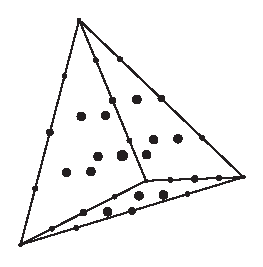
\includegraphics{figures/eps/tetra_popn.eps}}\hspace{4pt}
\caption{\textbf{Population points} }
\label{tetra_popn}
\end{center}
\end{figure}
Finite populations are represented by dots, 
where smaller dots have lower dispersion and are more likely points whereas larger dots have higher dispersion and are less likely points. 
The diagram also illuminates that finite populations are constrained to occupy lattice points 
within $\Lambda$. As population size $r \;\to\; \infty$, the lattice points become dense in $\Lambda$, 
which corresponds to the fact that an infinite population can be (represented by) any point of $\Lambda$.  

The variance of the next generation (with respect to the expected population) (see \cite{Vose1999}) is 
\begin{equation}
\label{RHSvariance}
\mathcal{E}(\| \tau (\bm{p}) - \mathcal{G}(\bm{p}) \|^2) = \frac{1 - \|\mathcal{G}(\bm{p})\|^2}{r}
\end{equation}

\section{Research Problems}
\begin{itemize}
\item{
Following Chebyshev's inequality (see \cite{ChebyshevInequality}) equation \ref{RHSvariance} becomes  
\begin{equation}
\label{Cheby}
P(\| \tau (\bm{p}) - \mathcal{G}(\bm{p}) \| \geq \epsilon) \leq \frac{1 - \|\mathcal{G}(\bm{p})\|^2} {r{\epsilon}^2}
\end{equation}
where $P$ above denotes probability and $\epsilon \;>\; 0$ is arbitrary.

Let $f(r)$ be a function which grows arbitrarily slowly, such that 
\[
\lim_{r \to \infty} f(r)  =  \infty
\]
and
\[
\lim_{r \to \infty} f(r)/\sqrt{r}  =  0.
\]
If 
\begin{equation}
\label{EpsilonCheby}
\epsilon  =  f(r)/\sqrt{r}
\end{equation}
then (\ref{Cheby}) becomes
\begin{equation*}
\lim_{r \to \infty} P(\| \tau (\bm{p}) - \mathcal{G}(\bm{p}) \| \geq \epsilon) \; \leq \; \lim_{r \to \infty}\frac{1 - \|\mathcal{G}(\bm{p}\|^2} {{f(r)}^2} \; = \; 0
\end{equation*}

Therefore, $\tau(\bm{p})$ converges in probability to $\mathcal{G}(\bm{p})$ as the population size increases, 
and $\tau$ corresponds to $\mathcal{G}$ 
in the infinite population case. Moreover, \ref{EpsilonCheby} suggests that the expected distance between finite and 
infinite population in the next generation might decrease as $1/\sqrt{r}$.

In figure \ref{tetra_popn}, finite population points can be only at certain points, but infinite population points can be anywhere in the simplex. 
Theorem 3.1 in `The Simple Genetic Algorithm: Foundations and Theory' states (see \cite{Vose1999}):  
\begin{quote}
\emph{If $\bm{p},\bm{q} \;\in\; \Lambda$ are 
arbitrary population vectors for population size $r$, and $\bm{\xi}$ denotes an arbitrary element of $\Lambda$, then 
\begin{eqnarray}
\underset{\bm{p} \neq \bm{q}}{\inf} \|\bm{p} - \bm{q}\| &\;=\;& \sqrt{2}/r    \label{theorem3.1_a} \\
\underset{\bm{\xi}}{\sup} \; \underset{\bm{p}}{\inf} \|\bm{\xi} - \bm{p}\| &\;=\;& O(1/\sqrt{r})     \label{theorem3.1_b}
\end{eqnarray}
where the constant (in the "big oh") is independent of the dimension $n$ of $\Lambda$}.
\end{quote}
From \ref{theorem3.1_b}, the distance between an infinite population $\bm{\xi}$ and finite population $p$ is $O(1/\sqrt{r})$. 
This suggests that the distance between $\tau (\bm{p})$ and $\mathcal{G}(\bm{p})$ might decrease as $1/\sqrt{r}$.

Let $\eta$ be the random variable $\| \tau (\bm{p}) - \mathcal{G}(\bm{p}) \|$, and let $\phi (x) = x^2$. 
% Then, $\mathcal{E}(\| \bm{q} - \mathcal{G}(\bm{p}) \|^2)$ becomes $\mathcal{E}(\phi (\eta))$. 
It follows from Jensen's Inequality (see \cite{JensenInequality}) that 
since $\phi$ is a convex function, 
\[
\phi(\mathcal{E}(\eta))) \leq \mathcal{E}(\phi(\eta)) 
\]
Therefore,
\begin{equation}
\label{Jensen}
\mathcal{E}(\| \tau (\bm{p}) - \mathcal{G}(\bm{p}) \|) \;=\; \mathcal{E}(\eta) \leq \sqrt{\mathcal{E}(\eta^2)} \;=\; \frac{\sqrt{1 - \|\mathcal{G}(\bm{p})\|^2}}{\sqrt{\bm{r}}}
\end{equation}
This suggests that the distance between $\tau (\bm{p})$ and $\mathcal{G}(\bm{p})$ might decrease as $1/\sqrt{r}$. 

Equations \ref{EpsilonCheby}, \ref{theorem3.1_b}, and \ref{Jensen} all suggest that the 
distance between $\tau(\bm{p})$ and $\mathcal{G}(\bm{p})$ might decrease as $1/\sqrt{r}$. 
All three of them are inequalities. The distance may decrease much faster than as $1/\sqrt{r}$ in reality. 
The first research question to consider is whether that rate of decrease can be exhibited 
in practice. We investigate the rate of decrease with experiments in Chapter 2.
}

\item{
An instance of RHS is {\em focused\/} if $\mathcal{G}$ is continuously differentiable, and for every $\bm{p}  \in  \Lambda$
the sequence
\[
\bm{p},  \mathcal{G}(\bm{p}),  {\mathcal{G}}^2(\bm{p}),...
\]
converges. In this case, $\mathcal{G}$ is also called focused, and the path determined by following at each generation what $\tau$ is expected 
to produce will lead to some fixed point $\omega$
\[
\mathcal{G}(\omega) = \lim_{n\to\infty} \mathcal{G}^n(\bm{p}) = \omega.
\]
When specialized to a simple GA (the details are explained in Chapter 2), it turns out that $ \mathcal{G}$ is focused under certain conditions, 
but under other conditions the sequence 
$\bm{p},  \mathcal{G}(\bm{p}),  {\mathcal{G}}^2(\bm{p}),...$ converges 
to a periodic orbit which oscillates between fixed points of $\mathcal{G}^2$ (see \cite{Vose1999}). 
If a finite population GA follows the infinite population GA closely, and if infinite populations oscillate under certain conditions, then 
finite populations might also show oscillating behavior. 
Akin analytically proves the existence of cycling for a continuous-time diploid two loci, two allele model (see \cite{Akin1982}). 
In contrast, we consider a discrete-time model with more than two loci. 
Hastings used a numerical approach to study 
the behavior of cycling populations with the infinite diploid population model (see \cite{Hastings1981}). 
His model includes crossover but not mutation. 
Moreover, the study was limited to two loci and two alleles. 
In contrast, we consider more than two loci, and include mutation. 
Wright and Bidwell provided examples when cycles in an infinite population model occur with mutation and 
crossover for 3 and 4 bit populations (see \cite{Wright1997}). 
Different behavior cases were observed. 
For a 3 bit example, both approximate period 2 cycling and long period cycling were observed. 
For a 4 bit example, long period cycling was observed. 
The examples provided were for specific 
parameter values. 
Their examples are based on computing a specific fitness function and a specific initial population from randomly generated 
mutation and crossover distributions in an attemp to find cyclic behavior anywhere within the parameter space of fitness, 
crossover and mutation. 
In contrast, we investigate cyclic behavior within a slice of the parameter space corresponding to fixed fitness, and consider 
randomly generated initial populations, as well as randomly generated crossover and mutation distributions.

\begin{figure}[h]
\begin{center}
\subfloat{
\resizebox{6cm}{5cm}{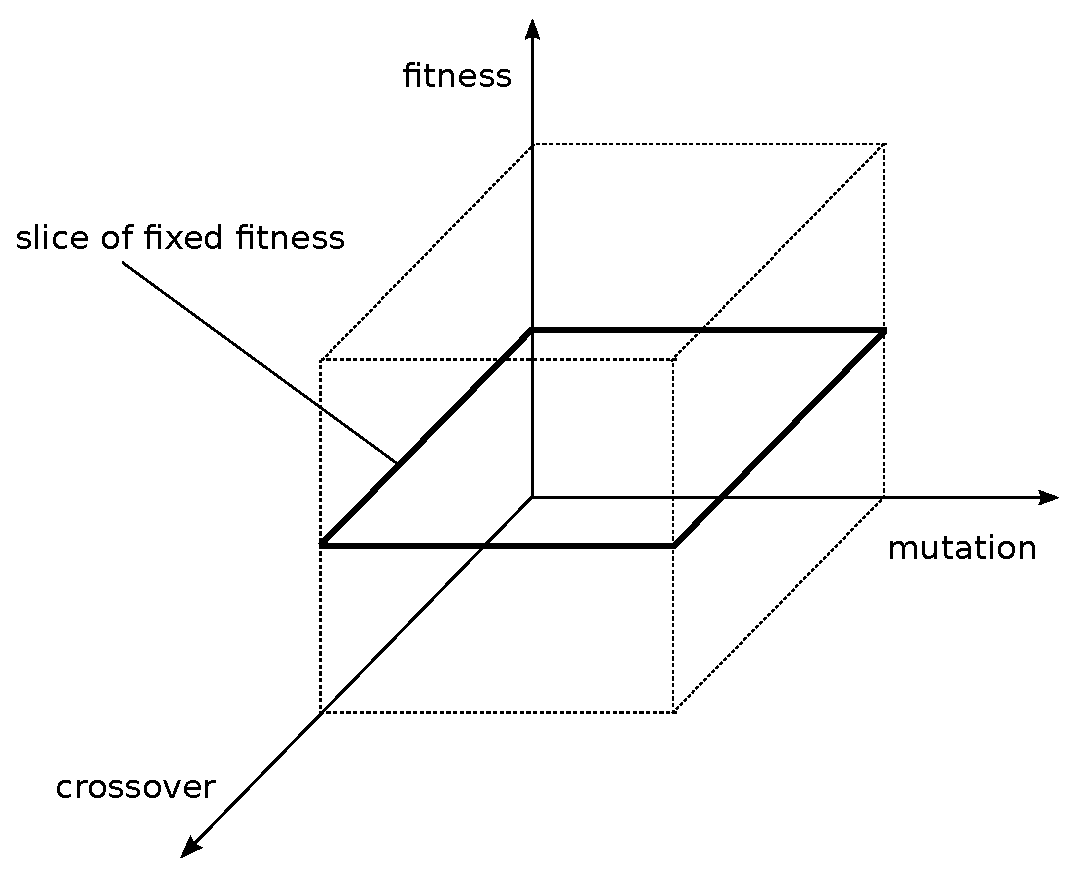
\includegraphics{figures/eps/cmf.eps}}}\hspace{-3em}%
\caption[\textbf{Parameter space of crossover, mutation and fitness}]{\textbf{Parameter space of crossover, mutation and fitness}  }
\label{fig_cmf}
\end{center}
\end{figure}

Similar in some respects to our approach, Wright and Agapie describe cycling behavior in one slice of 
the parameter space of fitness, crossover and mutation (see \cite{Wright2001}). 
They fix the fitness function to be one plus the integer value (of the population member).  
% Mutation used was density dependent mutation that uses separate mutation rate for each bit position. 
They showed results for 1-bit to 4-bit 
infinite population evolutions, and observed cyclic behavior of periods 2, 3, 4, 8 and 10. 
They also present data for finite populations exhibiting cyclic behavior. A significant difference between 
their investigation and ours is that their mutation is dynamic; the manner in which a population member mutates 
is dependent upon where the population is located in the state space $\Lambda$. In contrast, we consider static mutation which 
mutates population members uniformly irrespective of where the population is located in $\Lambda$. 
Moreover, works of Wright and Bidwell, and Wright and Agapie focus only on haploid population evolution 
whereas we consider both haploid and diploid population evolution.
Our research also studies cyclic behavior for a different slice of fitness   
than Wright and Agapie used in their work. 
We consider uniform fitness where every population member has the same fitness.
% but we vary crossover and mutation which are randomly generated. 
We find cycles in both finite and infinite population evolution, 
and provide visualization of oscillation related to infinite population fixed points. 
In Chapter 3, we investigate the second research question: Do 
finite populations exhibit oscillation in practice when infinite population oscillates? 
}

\item{
The third research question concerns the robustness of finite population oscillation.
Consider the lattice points in the simplex $\Lambda$ which represent finite populations 
(for some fixed population size $r$) 
and let $\bm{P}_j$ denote the $j$th population represented by the $j$th lattice point. 
Let $\bm{\pi}^k$ be the probability vector having as $j$th component 
the probability that $\bm{P}_j$ is the $k$th generation. 
If $\bm{\pi}^0$ is the initial population distribution, 
the steady state distribution $\bm{\pi}$ is given by (see \cite{Haggstrom2002})
\begin{equation}
\label{SteadyState}
\bm{\pi} \;=\; \lim_{k \to \infty} \bm{\pi}^k \;=\; \lim_{k \to \infty} \bm{\pi}^0 Q^k
\end{equation}
assuming the limit exists. The $j$th component $\bm{\pi}_j$ can be interpreted 
as the proporiton of time that a GA spends in population $\bm{P}_j$.
If transition matrix $Q$ is irreducible\footnote{A Markov chain is said to be 
{\em irreducible} if it is possible to get to any state from any state.} 
and aperiodic\footnote{A Markov chain is {\em aperiodic} if it can return to 
state $i$ at irregular times.}, then the Markov chain is 
regular (see \cite{Iosifescu1980}), the steady state distribution $\bm{\pi}$ exists, and it has positive components 
(see \cite{Minc1988}). 
The solution to equation \ref{SteadyState} satisfies
\begin{equation}
\label{SteadyStateSolution}
\bm{\pi} \; = \; \bm{\pi} Q
\end{equation}
where $\bm{\pi}$ is normalized so that its components sum to one.
If GA were to perfectly oscillate between two populations $\bm{P}_i$ and $\bm{P}_j$, then 
$\bm{\pi}^k_i \;=\; 1$ (other components are $0$) when $k$ is odd, 
and $\bm{\pi}^k_j \;=\; 1$ (other components are $0$) when $k$ is even. 
Therefore, perfect oscillation should not occur. In Chapter 4, we investigate oscillation behavior of 
finite populations when the Markov chain is regular. The third research question concerns whether 
finite population approximate oscillation can be exhibited in practice when the Markov chain is regular and 
infinite population trajectories have no periodic orbit.
}

\item{
In their work on cyclic behavior of populations, Wright and Agapie point out that the presence or 
absence of crossover did not affect cyclic behavior (see \cite{Wright2001}). 
But in our work, the condition for infinite population evolution to converge to periodic orbits depends upon crossover 
and if the crossover distribution condition is violated, infinite populations will not have periodic orbits (see \cite{Vose1999}). 
We investigate the robustness of finite population oscillation. 
The fourth research question is: Can finite population approximate oscillation be exhibited in practice when infinite population 
trajectories have no periodic orbit due to the crossover distribution violating the condition 
required for infinite population oscillation? 

}

\end{itemize}


% Equation \ref{Jensen} bounds the expected rate of convergence for the single-step haploid case; 
% the distance is inversely proportional to square root of population size. 
% Theorem 3.1 from 'The Simple Genetic Algorithm: Foundation and Theory', 
% and Jenson's inequality analysis of \ref{RHSvariance} both suggests that the distance between finite population and infinite population decreases like  
% $1\sqrt{r}$. We investigate the rate of decrease with experiments in Chapter 2. 
% We begin with a simple Markov model for diploid case under influence of mutation and crossover. 
% The model is non-overlapping, generational, infinite population model assuming random mating and no selective pressure. 
% Through abstract development, we show that the diploid model can be specialized by using mask based 
% mutation and crossover operators to Vose's infinite population model which is a haploid model. Computational 
% simplifications due to reduction of diploid model to haploid model and application of Walsh transform 
% are exploited in experimental simulation of model. Through the experiment we demonstrate convergence 
% of finite diploid population to infinite population behavior, and the distance between finite population 
% and infinite population decreases like $1\sqrt{r}$.

% We use computation of predicted limits
% of infinite population and present necessary and sufficient conditions stated by Vose for population
% to converge in to periodic orbits. We compute mutation distribution $\bm{\mu}$ and crossover distribution $\bm{\chi}$ 
% satisfying those conditions. Then, we study short-term behavior of finite population with respect to the limits to observe if oscillation occurs.

% If GA forms regular Markov chain visiting every population state infinitely often, then $\mathcal{G}$ is also called regular. 
% Let $\bm{P}_j$ denote $j$th population state in population state vector $P$. Let $\bm{\pi}^k$ be the probability vector having $j$th component 
% equal to the probability that $k$th generation population is $\bm{P}_j$. If $\bm{\pi}^0$ is initial distribution and $Q$ is transition matrix, the steady state distribution $\bm{\pi}$ is given by (see \cite{Nix1992})
% \[
% \lim_{k \to \infty} \bm{\pi}^k \;=\; \bm{\pi}^0 Q^k \;=\; \text{solution to the equation } "\bm{\pi} \; = \; \bm{\pi} Q" 
% \]
% where $j$th component can be interpreted as relative proporiton of time that GA has a population corresponding tp $\bm{P}_j$. 
% If the Markov chain is regular, then the steady state is independent of initial population. If GA were to converge to some population $\bm{P}_j$, 
% then $\bm{\pi}_j \;=\; 1$ and other components would be $0$. If GA were to oscillate between two populations $\bm{P}_i$ and $\bm{P}_j$, then 
% $\bm{\pi}_i \;=\; 1$ and other components $0$ when $k$ = odd generation, and $\bm{\pi}_j \;=\; 1$ and other components $0$ when $k$ = even generation. 
% But if GA forms regular Markov chain, this does not happen, instead finite population visits every population state infinitely often, and steady state 
% distribution $\bm{\pi}$ converges to $\bm{\pi}^\ast$ as population size increases to infinity ( see \cite{Nix1992}) where 
% \[
% \bm{\pi}^\ast \;=\; \lim_{r \to \infty} \bm{\pi}.
% \]
% So, in chapter three, we further investigate what happens to finite populations 
% if we violate the conditions necessary for population to oscillate, and making GA regular.

% If GA forms irreducible and aperiodic Markov chain, then the chain is regular (see \cite{MarkovChain}). 
% For regular Markov chain, 
% the steady state exists (it need not exist in general).  Hence, steady state distribution $\bm{\pi}$ 
% for regular Markov chain converges to some vector with positive values in its component, meaning oscillation 
% does not occur in GA if Markov chain is regular. In second part of Chapter 3, we further investigate 
% if finite populations approximately oscillate or not if regular Markov chain is formed. To study this, 
% we make some modifications in $\bm{\mu}$ and $\bm{\chi}$ distributions to  violate the conditions 
% necessary for population to oscillate such that GA will form regular Markov chain, and we observe finite 
% population short term behavior with this violation.

% \section{Overview}
% In chapter two, we describe a simple Markov model for diploid case under influence of mutation and crossover. 
% The model is non-overlapping, generational, infinite population model assuming random mating and no selective pressure. 
% Through abstract development, we show that the diploid model can be specialized by using mask based 
% mutation and crossover operators to Vose's infinite population model which is a haploid model. Computational 
% simplifications due to reduction of diploid model to haploid model and application of Walsh transform 
% are exploited in experimental simulation of model, and through the experiment we demonstrate convergence 
% of finite diploid population to infinite population behavior implied by equation \ref{RHSvariance}.
% 
% In chapter three, we study evolutionary limits predicted by Vose using infinite population model 
% under no selective pressure. We use computation of predicted limits
% of infinite population and present necessary and sufficient conditions stated by Vose for population
% to converge in to periodic orbits. We investigate predicting the convergence of finite population 
% short-term behavior to infinite population evolutionary limits under no selective pressure. 
% Then it studies case of violation in the necessary and sufficient conditions for population 
% to converge periodic orbits. We then study behavior of finite and infinite population when there is 
% violation in necessary condition mentioned by Vose.

% The genetic algorithm (GA) is inspired by nature, and seeks to evolve useful constructs. It is typically population based, and 
% proceeds over a number of generations to evolve solutions to problems not yielding to other known methods. 
% Basic elements of a GA are: 
% selection according to fitness, crossover, and random mutation (see \cite{Mitchell1999}). 
% In the simplest case, population members are fixed-length binary strings.   
% The fitness function assigns a score (fitness) to the elements (chromosomes) of 
% the current population. 
% 
% \textit{Selection}: select population members in the current population for reproduction; 
% those with higher fitness are more likely to be selected to reproduce.
% 
% \textit{Crossover}: with some probability (the crossover rate), choose a random point in two parents (population members selected for reproduction) 
% and exchange subsequences after that point to create two offspring.
% 
% \textit{Mutation}: flip bits of an individual with some small probability, 
% the mutation rate.
% 
% Figure \ref{FiniteGA} shows the procedural flow of a basic finite population genetic algorithm.
% \begin{figure}[H]
% \begin{center}
% \resizebox*{8cm}{!}{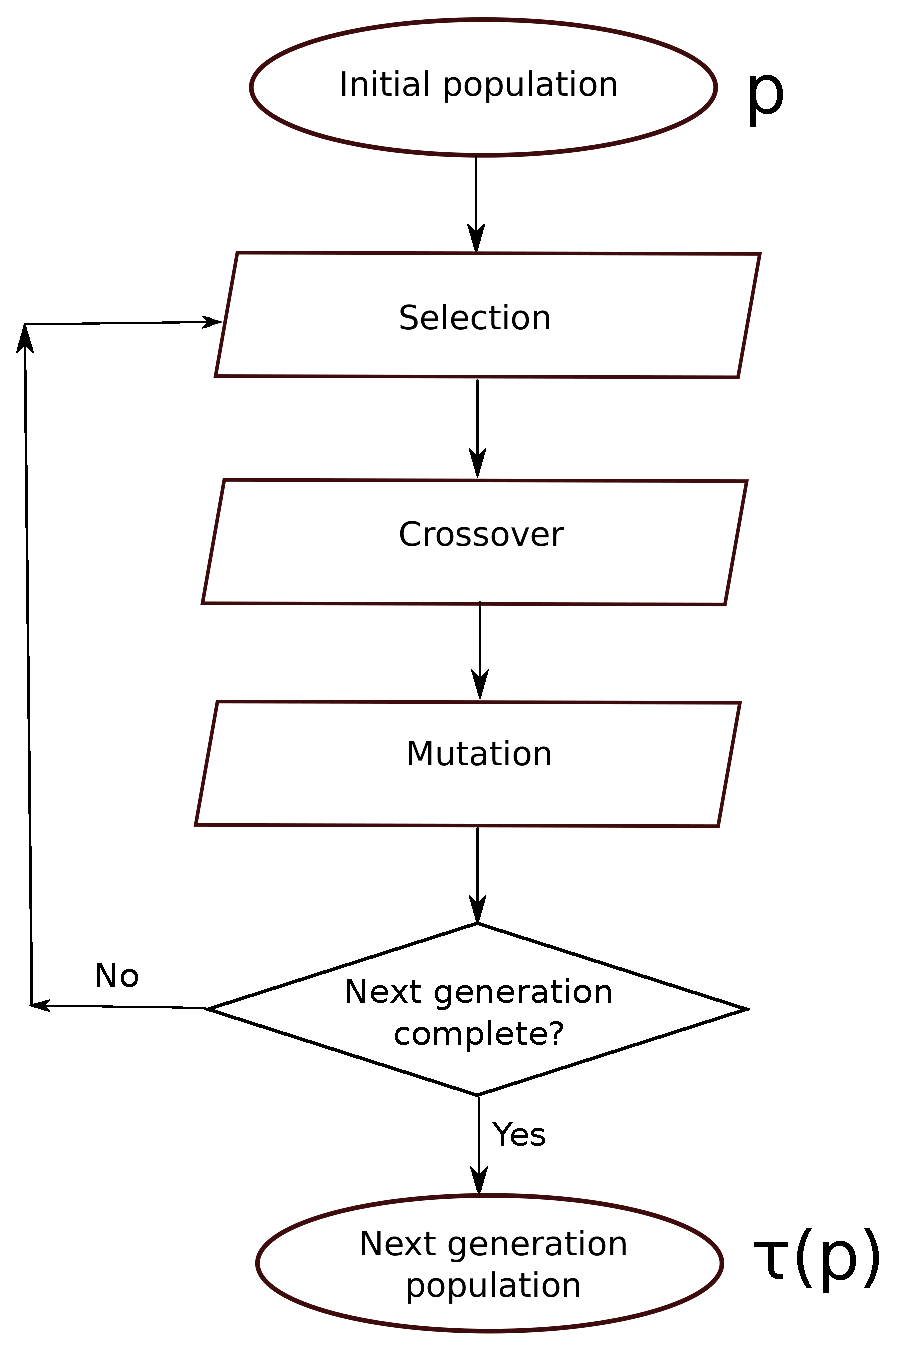
\includegraphics{figures/eps/GA.eps}}\hspace{4pt}
% \caption{\textbf{Finite GA (Haploid)} }
% \label{FiniteGA}
% \end{center}
% \end{figure}
% 
% A simple Holland style genetic algorithm (see \cite{Holland1975}):
% 
% \begin{algorithm}
% \caption*{}
% \begin{algorithmic}[1]
% \Statex 1. Start with some initial population $P$ containing $r$ binary strings of length $\ell$.
% \Statex 2. Choose (with replacement) parents $u$ and $v$ from the current population $P$ (using any selection scheme).
%   \Statex \hspace{\algorithmicindent} a. Cross $u$ and $v$ to produce children $u^\prime$ and $v^\prime$.
%   \Statex \hspace{\algorithmicindent} b. Mutate $u^\prime$ and $v^\prime$ with some probability to produce $u^{\prime\prime}$ and $v^{\prime\prime}$.
%   \Statex \hspace{\algorithmicindent} c. Keep, with uniform probability, one of $u^{\prime\prime}$ and $v^{\prime\prime}$ for the next generation 
% \Statex 3. If the next generation contains fewer than $r$ members, repeat step 2.
% \Statex 4. Replace $P$ by the new generation formed and go to step 2.
% \end{algorithmic}
% \label{RealGA}
% \end{algorithm}
% 
% Each iteration of this process produces a generation. 
% The process described above is repeated until the system stops to improve or some threshold is met. 
% 
% Figure \ref{FiniteGADip} illustrates 
% algorithm for finite diploid population genetic algorithm. 
% In case of diploid population GA each parent ($u$ or $v$) 
% has two haploid components ($\langle u_0, u_1 \rangle$ or $\langle v_0, v_1 \rangle$). 
% Instead of crossing over two parent diploids, 
% haploids in each diploid $u_0$ and $u_1$, and $v_0$ and $v_1$ 
% crossover and mutate to produce gametes $g_0$ and $g_1$ from  each diploid. 
% And gametes $g_0$ and $g_1$ are fused to form offspring diploid $ \langle g_0, g_1 \rangle $.
% 
% \begin{figure}[H]
% \begin{center}
% \resizebox*{8cm}{!}{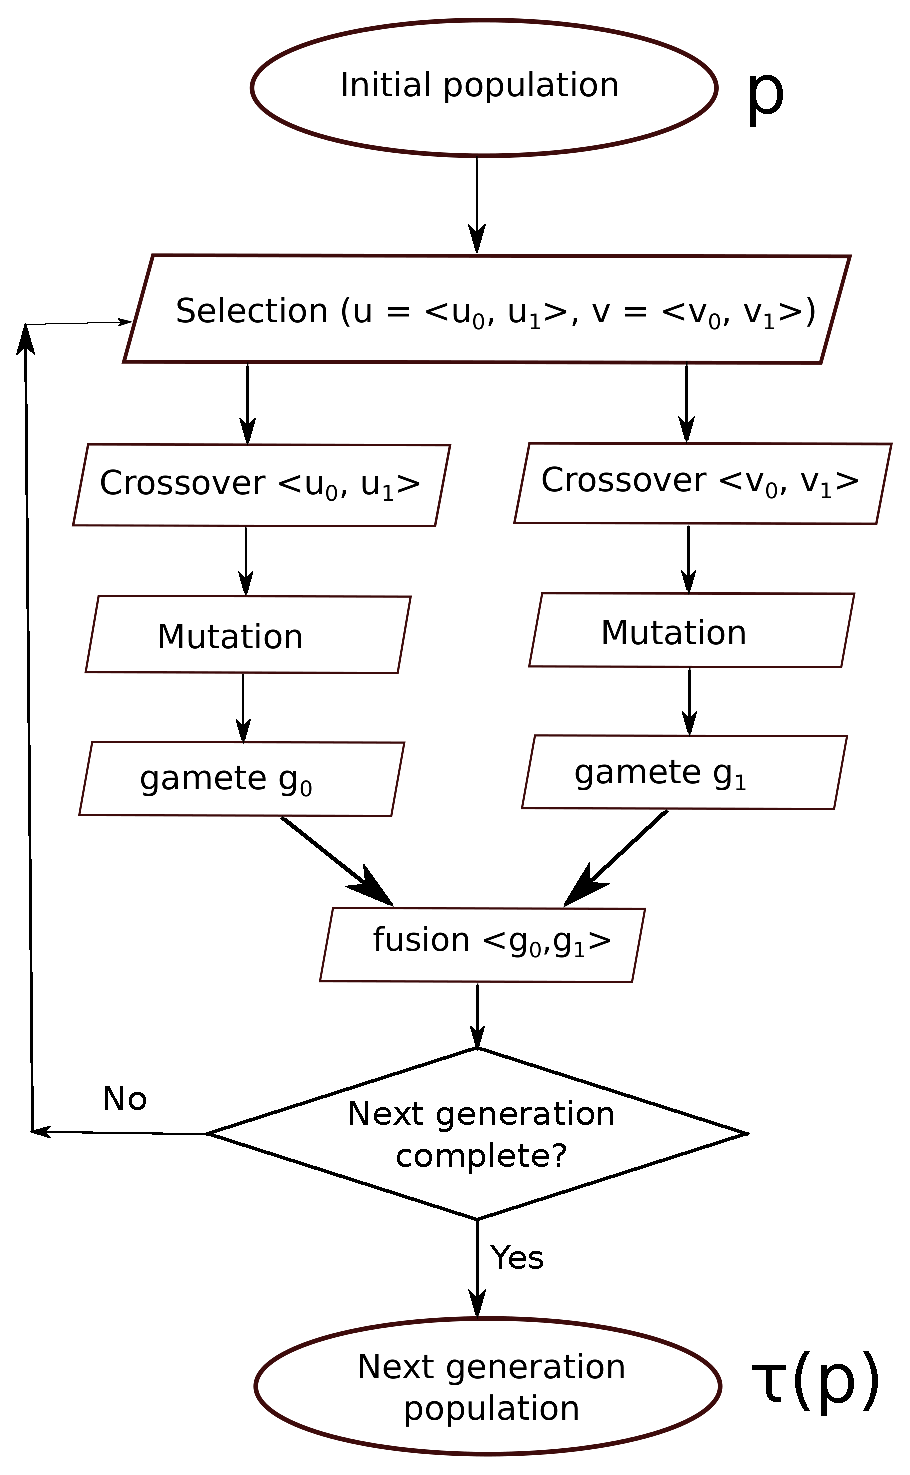
\includegraphics{figures/eps/GA_dip.eps}}\hspace{4pt}
% \caption{\textbf{Finite GA (Diploid)} }
% \label{FiniteGADip}
% \end{center}
% \end{figure}
% 
% 
% The infinite population GA models a population as a probability vector $\bm{p}$ where component $\bm{p}_j$ 
% can be interpreted as the proportion of string $j$ in the population. If $\mathcal{G}$ is the function mapping infinite population $\bm{p}$ to 
% the next generation, $\mathcal{G}(\bm{p})$ is a probability vector such that 
% \[
% \mathcal{G}(\bm{p})_j \; = \; \text{proportion of $j$ in the next generation}.
% \]
% The evolution of infinite population $\bm{p}$ is the sequence
% \[ \bm{p} \to \mathcal{G}(\bm{p}) \to  {\mathcal{G}}(\mathcal{G}(\bm{p})) \to \cdots \]
% \setcounter{footnote}{2}
% Haldane, in the classic book `The Causes Of Evolution', presents a summary of the basic models of population genetics 
% by Wright, Fisher, and Haldane (see \cite{Haldane1932}). 
% Several people working in the 1950s and the 1960s -- like Box (1957), Friedman (1959),
% Bledsoe (1961), Bremermann (1962), and Reed, Toombs and Baricelli (1967) -- developed evolution-inspired algorithms, 
% but little attention or theoretical analysis was given to them (see \cite{Mitchell1999}). Genetic algorithms were popularized by Holland 
% and his colleagues in the 1960s and the 1970s. Holland introduced a population-based algorithm with crossover and mutation, 
% and promoted his schema theorem ( see \cite{Holland1975}) as a theoretical means by which to analyze genetic algorithm dynamics. 
% Holland's Schema theorem provides a lower bound for schema survival in 
% next generation.\footnote{A schema is a template that identifies a set of strings in the population with similarities 
% at certain string positions; it is made up of $1$s, $0$s, and $\ast$s where 
% $\ast$ is the 'don't care' symbol that matches either $0$ or $1$.} The schema theorem is an inequality however, 
% and can not predict which strings are expected in the next generation. 
% Bethke (see \cite{Bethke1981}) gave equations computing the expected number of any string in the next generation. 
% Goldberg (see \cite{Goldberg1987}) used such equations 
% to model the evolutionary trajectory of a two bit GA under crossover 
% and proportional selection. Vose and Liepins (see \cite{VoseLiepins1991}) simplified and extended 
% these equations by integrating mutation into the recombination of arbitrarily long binary strings. 
% Although their model computes infinite population trajectories, given a {\em finite} population represented by vector $\bm{p}$  
% (component $\bm{p}_i$ is the proportion of string $i$ in the {\em finite population}), the infinite population model 
% computes the expected proportion $\mathcal{G}(\bm{p})_i$ of string $i$ in the next generation.  This is perhaps the most 
% direct connection between the infinite population model and a finite population GA.
% 
% Nix and Vose (see \cite{Nix1992}) explored issues regarding the relationship between the finite population GA and the infinite population model. 
% For a mutation rate $\mu$ between $0$ and $0.5$, a finite population GA will form an ergodic Markov chain, 
% visiting every state infinitely often in the long run.
% The short term trajectory followed by a finite population is related to 
% the evolutionary path determined by the infinite population model. 
% For large populations, the short term trajectory follows closely and 
% with large probability, that path predicted by 
% the infinite population model. 
% % So if we form a geometrical cylinder 
% % around the path determined by the infinite population model, a finite population GA will stay inside the pipe in the short term, and 
% % then escape it after some period of time. 
% 
% % Vose and Liepins apply Walsh transform to mixing to analyse and get results. 
% % With Markov chain modeling of simple GA, Vose and Nix (see \cite{Nix1992}) investigated asymptotic behavior of steady 
% % state distributions as population size increases and showed that if finite population is sufficiently large, 
% % convergence behavior of a real GA can be predicted. As population size increases, the correspondence improves 
% % between expected population predicted using infinite population model and the actual population observed in 
% % finite population genetic algorithm. 
% 
% Vose compiled and extended previous work regarding the infinite population model in the book 
% \textit{Simple Genetic Algorithm: Foundations and Theory} (see \cite{Vose1999}). 
% In particular, he discussed how the Walsh transform can be applied to increase 
% computational efficiency in calculations related to the infinite population model. 
% There have been previous applications of the Walsh transform to GAs. Bethke first introduced the 
% idea of using Walsh transforms to analyze GA fitness functions in terms of schemata (see \cite{Bethke1981}). 
% The idea was further developed in papers by Goldberg (see \cite{Goldberg1989a}, \cite{Goldberg1989b}). 
% However, such usage did not apply Walsh transforms  to crossover, to mutation, or to any of their 
% associated mathematical objects. In contrast, Vose and Liepins applied the Walsh transform directly to mutation and recombination, and proved that the 
% twist $M^\ast$ of the mixing matrix $M$ is triangularized by the Walsh transform, and 
% related eigenvalues of $M^\ast$ to the stability of fixed points of $\mathcal{G}$ (see \cite{VoseLiepins1991}).\footnote{The mixing 
% matrix $M$ has rows and columns indexed by chromosomes; entry $M_{i,j}$ is the probability 
% that mixing parents $i$ and $j$ (mixing is the combined effect of crossover and mutation) will produce a 
% child having all bits zero. The twist $(M^\ast)$ of the mixing matrix $M$ is defined by $(M^\ast)_{i,j} = M_{i+j, i}$.} 
% In a related paper, Koehler (see \cite{Koehler1994}) gives a congruence 
% transformation defined by a lower triangular matrix that diagonalizes the mixing matrix (for 1-point crossover and mutation 
% given by a rate) and proved a conjecture of Vose and Liepins concerning eigenvalues of $M^\ast$. Koehler, Bhattacharyya 
% and Vose (see \cite{KoehlerBhatta1997}) applied the Fourier transform in generalizing results established 
% for binary GAs to 
% strings over an alphabet of cardinality $c$ (in the binary case, the Fourier transform is the Walsh transform). 
% From a computational perspective, a major contribution of Vose and Wright (see \cite{VoseWright1998}) was demonstrating that 
% the mixing matrix is sparse in the Walsh basis, and the computational efficiency of 
% computing $\mathcal{G}(\bm{p})$ can thereby be improved from 
% $O(8^\ell)$ to $O(3^\ell)$ where $\ell$ is the chromosome length. The cost of moving from standard coordinates to the Walsh basis need not be a bottleneck; 
% the fast Walsh transform (see \cite{Shanks1969}) does that in $O(\ell \, 2^\ell)$ time.
% 




